%
% Complete documentation on the extended LaTeX markup used for Insight
% documentation is available in ``Documenting Insight'', which is part
% of the standard documentation for Insight.  It may be found online
% at:
%
%     http://www.itk.org/

\documentclass{InsightArticle}

\usepackage[dvips]{graphicx}
\usepackage{float}
\usepackage{subfigure}
\usepackage{amsmath} % for cases{}
\usepackage{graphicx}

%%%%%%%%%%%%%%%%%%%%%%%%%%%%%%%%%%%%%%%%%%%%%%%%%%%%%%%%%%%%%%%%%%
%
%  hyperref should be the last package to be loaded.
%
%%%%%%%%%%%%%%%%%%%%%%%%%%%%%%%%%%%%%%%%%%%%%%%%%%%%%%%%%%%%%%%%%%
\usepackage[dvips,
bookmarks,
bookmarksopen,
backref,
colorlinks,linkcolor={blue},citecolor={blue},urlcolor={blue},
]{hyperref}


\title{Poisson Editing in ITK}

% 
% NOTE: This is the last number of the "handle" URL that 
% The Insight Journal assigns to your paper as part of the
% submission process. Please replace the number "1338" with
% the actual handle number that you get assigned.
%
\newcommand{\IJhandlerIDnumber}{3257}

% Increment the release number whenever significant changes are made.
% The author and/or editor can define 'significant' however they like.
\release{0.00}

% At minimum, give your name and an email address.  You can include a
% snail-mail address if you like.

\author{David Doria}
\authoraddress{Rensselaer Polytechnic Institute, Troy NY}


\begin{document}

%
% Add hyperlink to the web location and license of the paper.
% The argument of this command is the handler identifier given
% by the Insight Journal to this paper.
% 
\IJhandlefooter{\IJhandlerIDnumber}


\ifpdf
\else
   %
   % Commands for including Graphics when using latex
   % 
   \DeclareGraphicsExtensions{.eps,.jpg,.gif,.tiff,.bmp,.png}
   \DeclareGraphicsRule{.jpg}{eps}{.jpg.bb}{`convert #1 eps:-}
   \DeclareGraphicsRule{.gif}{eps}{.gif.bb}{`convert #1 eps:-}
   \DeclareGraphicsRule{.tiff}{eps}{.tiff.bb}{`convert #1 eps:-}
   \DeclareGraphicsRule{.bmp}{eps}{.bmp.bb}{`convert #1 eps:-}
   \DeclareGraphicsRule{.png}{eps}{.png.bb}{`convert #1 eps:-}
\fi


\maketitle


\ifhtml
\chapter*{Front Matter\label{front}}
\fi


% The abstract should be a paragraph or two long, and describe the
% scope of the document.
\begin{abstract}
\noindent
This code provides an implementation of two techniques from ``Poisson Image Editing'' on ITK images. First, we fill a hole in an image given only the pixel values on the boundary. Second, we copy a region of an image into another image and make the result as smooth as possible. We also explain how these techniques can be used to reconstruct an image after perform editing operations in the gradient domain. The code is available here: https://github.com/daviddoria/PoissonEditing

\end{abstract}

\IJhandlenote{\IJhandlerIDnumber}

\tableofcontents

%%%%%%%%%%%%%%%%%
\section{Introduction}
This code provides an implementation of two techniques from ``Poisson Image Editing'' \cite{PoissonImageEditing} on ITK images. First, we fill a hole in an image given only the pixel values on the hole boundary. Second, we copy a patch of an image into another image and make the resulting image as smooth as possible. The code is available here: https://github.com/daviddoria/PoissonEditing

%%%%%%%%%%%%%%%%%
\section{Hole Filling}
As a motivating example of the power of Poisson methods in image editing, we attempt to fill in a missing region in an image in a plausible way. In this example, our goal is to remove the jet from the image in Figure \ref{fig:HoleFilling:original}. To do this, we must manually specify the region to be removed (shown in Figure \ref{fig:HoleFilling:mask}). The result of the filling is shown in Figure \ref{fig:HoleFilling:filled}.

\begin{figure}[H]
\centering
\subfigure[Original image]{
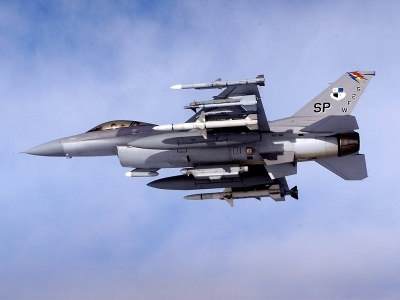
\includegraphics[width=0.3\linewidth]{images/plane}
\label{fig:HoleFilling:original}
}
\subfigure[Mask]{
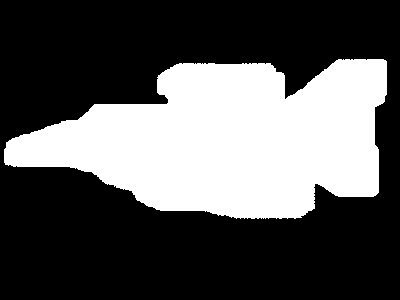
\includegraphics[width=0.3\linewidth]{images/planeMask}
\label{fig:HoleFilling:mask}
}
\subfigure[Filled image]{
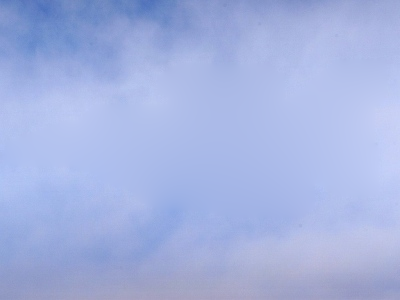
\includegraphics[width=0.3\linewidth]{images/planeFilled}
\label{fig:HoleFilling:filled}
}
\caption{A demonstration of Poisson hole filling}
\label{fig:HoleFilling}
\end{figure}

\subsection{Input}
The inputs to this algorithm are:
\begin{itemize}
\item An image, $I$.
\item A mask indicating the region to fill. The mask must be the same size as the image, and must not have non-zero pixels on its border.
\end{itemize}

\subsection{Concept}
It has been shown using Calculus of Variations that the best solution for the region inside the hole, $H$, is given by the solution to 

\begin{equation}
\nabla^2 H = 0
\end{equation}

while ensuring $H=I$ on the boundary of the hole. This setup is a Laplace equation with Dirichlet (a.k.a. first order) boundary conditions. 

\subsection{Discrete Solution}
The Laplace operator is given by
\begin{equation}
 \nabla^2 f = \sum_{i=1}^n \frac{\partial^2 f}{\partial x_i^2}
\end{equation}

A discrete approximation to this function at a pixel $(x,y)$ is given by
\begin{equation}
 \nabla^2 f(x,y) \approx f(x-1,y) + f(x+1,y) + f(x,y-1) + f(x,y+1) - 4f(x,y).
\end{equation}

Another way to write this is to multiply the pixel and its neighbors by the kernel shown in \ref{eqn:kernel}.
\begin{equation}
\label{eqn:kernel}
\begin{pmatrix}
0 & 1 & 0 \\
1 & -4 & 1\\
0 & 1 & 0
\end{pmatrix}
\end{equation}


For each unknown pixel $u_{i,j}$, the equation is therefore

\begin{equation}
\label{eqn:DiscreteLaplacian}
-4 u_{i,j} + u_{i+1,j} + u_{i-1,j} + u_{i,j+1} + u_{i,j-1} = 0.
\end{equation}

To solve the Laplace equation over the entire image, we can write a linear system of equations. We create a variable for every pixel to be filled. If the pixels are vector-valued (e.g. an RGB image), $N$ of these systems must be solved independently (where $N$ is the dimensionality of each pixel).

A sparse matrix $U$ is constructed row by row, one row per variable. In each row, the value in the Laplacian kernel corresponding to the pixel's location relative to the current variable pixel is placed in the column corresponding to the variable id. When one of the pixels appearing in Equation \ref{eqn:DiscreteLaplacian} is on the border of the hole (and is therefore known), $u_{(\cdot,\cdot)}$ is replaced with $p_{(\cdot,\cdot)}$, the value of the pixel from the original image. In this case, rather than place the value of the Laplacian kernel in the $U$ matrix, we instead multiply it by the image value and subtract the result from the corresponding entry of the $b$ vector. That is, we move the known value to the right side of the equation.

A vector $H_v$, the vectorized version of the solution to the set of hole pixels, is created as the unknown vector to be solved in a system of equations.

The linear system is then
\begin{equation}
 U^T H_v = b.
\end{equation}

After solving for $H_v$, the resulting $H_v$ is then remapped back to the pixels corresponding to each variable id to construct $H$. $U$ is incredibly sparse, so a sparse solver should definitely be used.

\subsection{Code Snippet}
We have packaged this implementation in a class called $PoissonEditing$. Using this class is very straight forward. The $TargetImage$ and $Mask$ must be set. The class is designed to operate on scalar images. As we typically want to operate on color images, or generally images with pixels of length $N$, we provide static helper functions which decompose the input image, perform the Poisson filling/cloning operation on each channel individually, and reassemble the final output.

Below we show the use of one of these helper functions (as this is typically the case that the end user will use). We note the use of the $zeroGuidanceField$ object. Though we have not yet explained this concept, we will see in the next section that the Poisson hole filling problem is simply a degenerate case of the more general Poisson Cloning problem where the guidance field is set to zero. Furthermore, we must pass the full region of the target image indicating that we will be filling the hole where it is currently located. The reason for this will be clear once we show in the next section that we can position the source image anywhere in the target image for the Poisson Cloning problem.

\begin{verbatim}
PoissonEditing<float>::FillImage(targetImage, mask,
				 zeroGuidanceField.GetPointer(), output,
				 targetImage->GetLargestPossibleRegion());
\end{verbatim}


%%%%%%%%%%%%%%%%%
\section{Region Copying/Poisson Cloning}
\label{sec:RegionCopying}
In the problem of region copying (a.k.a. seamless cloning or Poisson cloning), we are interested in copying a region from one image into another image in a visually pleasing way. This is again best motivated with an example. In our example, the goal is to copy the jet from Figure \ref{fig:RegionCopying:original} into the image of the canyon shown in Figure \ref{fig:RegionCopying:target}. This source and target pair along with the mask and the result are shown in \ref{fig:RegionCopying}.

\begin{figure}[H]
\centering
\subfigure[Original image]{
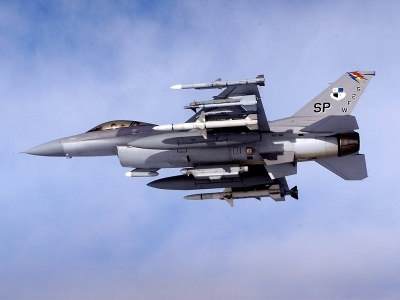
\includegraphics[width=0.2\linewidth]{images/plane}
\label{fig:RegionCopying:original}
}
\subfigure[Mask]{
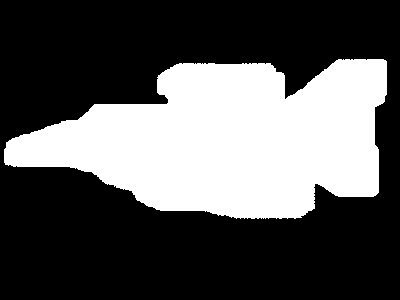
\includegraphics[width=0.2\linewidth]{images/planeMask}
\label{fig:RegionCopying:mask}
}
\subfigure[Target Image]{
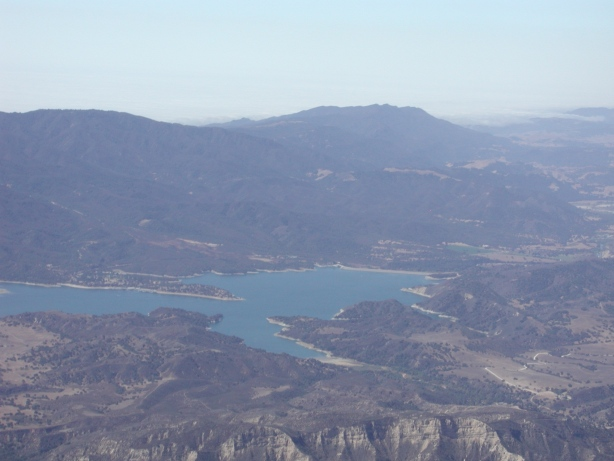
\includegraphics[width=0.2\linewidth]{images/planeTarget}
\label{fig:RegionCopying:target}
}
\subfigure[Resulting Image]{
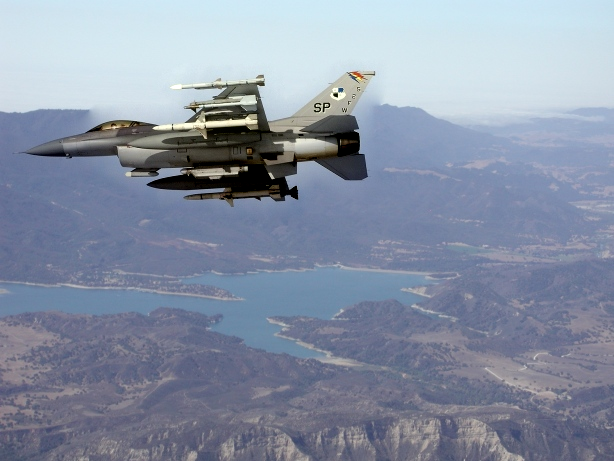
\includegraphics[width=0.2\linewidth]{images/planeCopyingResult}
\label{fig:RegionCopying:result}
}
\caption{A demonstration of Poisson region copying}
\label{fig:RegionCopying}
\end{figure}

\subsection{Input}
The inputs to this algorithm are:
\begin{itemize}
\item A source image, $S$.
\item A target image, $T$.
\item A mask, $M$, indicating the region to fill. The mask must be the same size as the image, and must not have non-zero pixels on its border.
\end{itemize}

\subsection{Concept}

In \cite{PoissonImageEditing}, it was argued that a good way to copy a region of one image into another image is to do something very similar to hole filling, but additionally introduce a ``guidance field'', $G$. That is, the way to copy a region of one image into another is to solve the equation

\begin{equation}
\nabla^2 H = div(G).
\end{equation}

The boundary condition this time is again first order and specifies that the resulting $H$ be equal to the target image, $T$, at the hole boundary.

The suggested guidance field $G$ is the gradient of the source image. That is,

\begin{equation}
G = \nabla S.
\end{equation}

In this case, the right hand side of the equation has become $div(\nabla S)$, which is exactly the Laplacian of $S$.

\subsection{Discrete Solution}
Just as before, the discrete Laplacian equation is written for each pixel, but this time the right hand side is set to $\nabla^2 S(i,j)$ as shown in \ref{eqn:DiscretePoisson}. When the right side of this equation is non-zero, it is referred to as a Poisson equation.

\begin{equation}
\label{eqn:DiscretePoisson}
-4 u_{i,j} + u_{i+1,j} + u_{i-1,j} + u_{i,j+1} + u_{i,j-1} \approx \nabla^2 S(i,j)
\end{equation}

The linear system 
\begin{equation}
 U^T H_v = b
\end{equation}

is created and solved identically as before.

\subsection{Positioning the Source Image in the Target Image}
The source image is assumed to be smaller than the target image. By default, the source image is composited in the top right of the target image. However, we can position the source image anywhere on the target image as long as the moved source image is completely inside the target image. We do this using the $SetRegionToProcess(itk::ImageRegion)$ function.

\subsection{Code Snippet}
This functionality can be used almost identically as in the last section, but a TargetImage must be specified:

\begin{verbatim}
  itk::ImageRegion<2> regionToProcess = ...; // specify where in the target image the source image should be composited.
  
  PoissonEditingType::FillImage(targetImageReader->GetOutput(), mask,
                                guidanceFields, outputImage.GetPointer(), regionToProcess);
\end{verbatim}

%%%%%%%%%%%%
\section{Manipulation in the Gradient Domain}
There are tricks that can be done by performing operations to the derivatives of an image. The goal of such manipulations is often to produce an effect in the original image. To get back to the image from the gradient, one must find the least squares solution to a system of equations involving the derivatives of the image (see Section \ref{sec:ReconstructingFromDerivatives}). However, this technique is not often used. More commonly, the derivatives are recombined into the Laplacian and the reconstruction is done using the methods described in previous sections. We will outline both techniques below.

\subsection{Reconstructing an Image from Its Derivatives}
\label{sec:ReconstructingFromDerivatives}
For the task of reconstructing an image directly from its derivatives, we can use a very similar method to solving the Laplace equation. This time, however, there are two equations to be solved simultaneously:
\begin{align}
\frac{dU}{dx} &= D_x \\
\frac{dU}{dy} &= D_y
\end{align}

where $D_x$ and $D_y$ are the known derivative images and $U$ is the unknown image. Of course the first order boundary conditions must again be known. This time the boundary is the actual border of the image.

We can construct the same type of linear system to solve for the components of $U$ that best satisfy both equations. Any discrete derivative operator can be used. We have chosen to use the Sobel operators:

\begin{figure}[H]
  \begin{minipage}[b]{0.5\linewidth}
    \centering

    \begin{equation}
    S_x =
    \begin{pmatrix}
    -1 & 0 & 1 \\
    -2 & 0 & 2\\
    -1 & 0 & 1
    \end{pmatrix}
    \end{equation}

  \end{minipage}
    \hspace{0.5cm}
  \begin{minipage}[b]{0.5\linewidth}

    \begin{equation}
    S_y =
    \begin{pmatrix}
    -1 & -2 & -1 \\
    0 & 0 & 0\\
    1 & 2 & 1
    \end{pmatrix}
    \end{equation}

  \end{minipage}
\end{figure}

By applying these operators to every pixel in $U$, we can write a system of equations, two equations for each pixel as shown below.

\begin{align}
- u_{i-1,j-1} -2 u_{i-1,j} - u_{i-1,j+1} + u_{i+1,j+1} + 2 u_{i+1,j} + u_{i,j+1} &= D_x(i,j) \\
- u_{i-1,j-1} -2 u_{i,j-1} - u_{i+1,j+1} + u_{i-1,j-1} + 2 u_{i,j+1} + u_{i+1,j+1} &= D_y(i,j)
\end{align}

Again, we simply place the coefficient of each term in the column of the matrix corresponding the variable id of the pixel. As usual, we move the term to the right side of the equation (to contribute to the $b$ vector) if the pixel is known. Figure \ref{fig:DerivativeReconstruction} shows an image, its derivatives, and the image reconstructed using only the border of the image in \ref{fig:DerivativeReconstruction:original} and the derivatives.

\begin{figure}[H]
\centering
\subfigure[Original image]{

\includegraphics[width=0.2\linewidth]{images/smiley}
\label{fig:DerivativeReconstruction:original}
}
\subfigure[$D_x$]{

\includegraphics[width=0.2\linewidth]{images/smileyXDerivative}
\label{fig:DerivativeReconstruction:mask}
}
\subfigure[$D_y$]{

\includegraphics[width=0.2\linewidth]{images/smileyYDerivative}
\label{fig:DerivativeReconstruction:target}
}
\subfigure[Resulting Image]{

\includegraphics[width=0.2\linewidth]{images/smileyReconstructed}
\label{fig:DerivativeReconstruction:result}
}
\caption{A demonstration of reconstructing an image from its derivatives}
\label{fig:DerivativeReconstruction}
\end{figure}

\subsubsection{Implementation}
We have provided this implementation in a file called $DerivativesToImage.cxx$.

\subsection{Reconstructing an Image from Its Laplacian}
\label{sec:ReconstructingFromLaplacian}
The technique to reconstruct an image from its Laplacian is identical to the procedure described in Section \ref{sec:RegionCopying}. We specify the Laplacian in the unknown region as the guidance field. If the manipulation was done directly on the Laplacian, this process was straight forward. However, if the manipulation was done on the derivative images, there is an additional step of going from the derivatives to the Laplacian that requires special attention.

The Laplacian is defined as the divergence of the gradient, which can be written as

\begin{equation}
\nabla^2 I = div(\nabla I).
\end{equation}

In this case, we know the gradient,
\begin{equation}
\nabla I (i,j) = (D_x(i,j), D_y(i,j)) 
\end{equation}

so the Laplacian is 
\begin{equation}
\nabla I^2(i,j) = \frac{\partial D_x(i,j)}{\partial x} + \frac{\partial D_y(i,j)}{\partial y}.
\end{equation}

That is, we must take the $x$ derivative of the $x$ derivative that we already have, and the $y$ derivative of the $y$ derivative that we already have, and add them together. NOTE: the discrete operators that you choose is critically important. If you use the 5 points Laplacian operator

\begin{equation}
\begin{pmatrix}
0 & 1 & 0 \\
1 & -4 & 1\\
0 & 1 & 0
\end{pmatrix}
\end{equation}

you MUST use the forward difference operator (shown in \ref{eqn:ForwardDifference}) to take the first set of derivatives (which produce the input to the algorithm).

\begin{figure}[H]
\label{eqn:ForwardDifference}
  \begin{minipage}[b]{0.5\linewidth}
    \centering

    \begin{equation}
    \begin{pmatrix}
    0 & 0 & 0 \\
    0 & -1 & 1\\
    0 & 0 & 0
    \end{pmatrix}
    \end{equation}

  \end{minipage}
    \hspace{0.5cm}
  \begin{minipage}[b]{0.5\linewidth}

    \begin{equation}
    \begin{pmatrix}
    0 & 0 & 0 \\
    0 & -1 & 0\\
    0 & 1 & 0
    \end{pmatrix}
    \end{equation}
  \end{minipage}
\end{figure}

Similarly, the backward difference operator that must be used to take the second derivatives is

\begin{figure}[H]
  \begin{minipage}[b]{0.5\linewidth}
    \centering

    \begin{equation}
    \begin{pmatrix}
    0 & 0 & 0 \\
    -1 & 1 & 0\\
    0 & 0 & 0
    \end{pmatrix}
    \end{equation}

  \end{minipage}
    \hspace{0.5cm}
  \begin{minipage}[b]{0.5\linewidth}

    \begin{equation}
    \begin{pmatrix}
    0 & -1 & 0 \\
    0 & 1 & 0\\
    0 & 0 & 0
    \end{pmatrix}.
    \end{equation}

  \end{minipage}
\end{figure}

It possible to choose different operators, but you must choose the derivative operators so that if they are applied successively they produce exactly the Laplacian operator that you choose. If you do not do this, the result of the reconstruction will be wildly incorrect.

We have provided this implementation in a file called $LaplacianToImage.cxx$.

%%%%%%%%%%%%
\section{Notes}
\subsection{Clamping outputs}
It is important to note that everywhere in this document the linear systems have been solved with no constraints. This allows the resulting image to take invalid values (i.e. greater than 255 or less than 0). The resulting images must therefore be clamped or scaled to ensure the output has an appropriate range.

\subsection{Efficiency}
The hole filling example in this document took only 0m1.5s. The computation is done using the SimplicialLDLT solver from the Eigen library.

\bibliography{InsightJournal}
\bibliographystyle{plain} % MUST include this line or will get ``undefined reference'' errors

\end{document}

